\chapter{Interactivity}

The \verb|sidBison| tool cannot be considered a successful stepwise debugger if it is not truly interactive. As a result, each command must execute in a resonable amount of time. Since a command's execution time may be context dependent, an understanding of the system's time-complexity may help users improve their use of the system. These analytical formulae, along with empirical run-times,
also allow for the evaluation of the interactivity of \verb|sidBison|.

\section{Complexity}

\paragraph{Complexity of Bison}

It is necessary to understand the runtime of Bison before reasoning about \verb|sidBison|'s runtime. According to the Bison user manual, "a GLR parser can take quadratic or cubic worst-case time, and the current Bison parser even takes exponential time and space for some grammars" \cite{LinearBison}. However, for most grammars parsing time is $O(|G| n)$ \cite{LinearBison}\cite{ComplexityGLR}. $|G|$ is the number of tokens in the grammar and $n$ is the length of the string to be parsed.

\paragraph{Reading from iBison}

\verb|sidBison| is built on top of Satya Kiran Popuri's \verb|iBison| system. As a result, much of \verb|sidBison|'s resources and run-time are invested in inter-process communication. Several commands read information from the iBison process. As a result, it is important to compute the asymptotic time needed to communicate with iBison.

\begin{enumerate}
\item  The size of information output from \verb|iBison| is a function of its state and token stack sizes.
\item \verb|sidBison| sets an upper limit of $1 KB$ on the sizes of the state and token stacks.
\item As a result, there is a fixed upper bound on the information that needs to be read from iBison.
\end{enumerate}

Thus, while the constants in question may be large (at most $2 KB$), reading information from iBison takes $O(1)$ time.
This communication is implemented in the  function \verb|read_from_ibison|.

\paragraph{step}

The \verb|step| command is the most basic of \verb|iBison| commands. It executes a single Bison step. Since reading from iBison takes constant time, \verb|step|'s run-time has complexity $O(n|G|)$ where $n = 1$. Since the number of tokens in a grammar is constant for any debugging instance, step runs in constant time. 

\paragraph{steprule}

The \verb|steprule| command steps repeatedly till a reduce action is executed. Thus, it may call \verb|step| up to $n$ times, where $n$ is the length of the input string. As a result, since the number of tokens in a grammar is constant for any debugging instance, it has complexity $O(n)$.

\paragraph{ctkn}

The \verb|ctkn| command accesses the newer of the top element of the token stack and the lookahead to return the current token. As both these operations take constant time, \verb|ctkn| runs in $O(1)$.

\paragraph{str}

The \verb|str| command returns the contents of the token stack. As the size of this stack is bounded, it runs in $O(1)$.

\paragraph{br}

The \verb|br| command steps repeatedly till the current token equals a specified token. Thus, it may call \verb|step|  and \verb|ctkn| up to $n$ times each, where $n$ is the length of the input string. As both \verb|step| and \verb|ctkn| take constant time, it has complexity $O(n)$.

\paragraph{crule}

The time-travelling \verb|crule| command spawns a new \verb|iBison| process and steps first to the current state, and then till the current rule is reduced. As a result, it steps and reads from iBison  up to $n$ times, where $n$ is the length of the input string. As a result, it runs in $O (n)$. However, given that it has to spawn a new process, the constants in the linear describing its execution time are large.

\paragraph{rulepos}

The \verb|rulepos| command helps identify the user's current position in the rule they are parsing. It first looks up the rules associated with the current parser automaton state and then calls \verb|crule|. As looking up rules is a constant time operation, and \verb|crule| is linear, the \verb|rulepos| command runs in $O(n)$.\\



\section{Empirical analysis}

Compiling \verb|sidBison| with the \verb|DDEBUGLOG=1| flag enables a timing routine with least count $10^{-6}$ seconds . This feature writes system and user time taken by a command to \verb|stderr|. Runtimes for each command were logged while debugging examples in Appendix C. Raw data can be found in Appendix D.



\begin{figure}[H] \centering
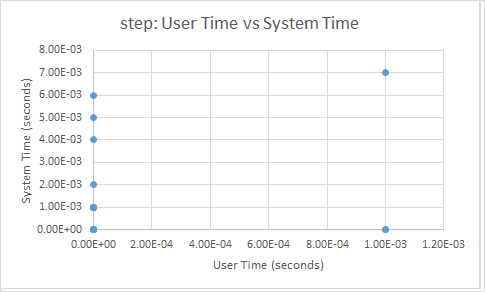
\includegraphics[height=6cm,width=10cm]{step.png}
\end{figure}

\noindent

The average user time taken by the \textbf{step} command was $1.07*10^{-4}s$ with standard deviation $3.150 * 10^{-4} s$. The average system  time taken was $1.29*10^{-3} s$ with standard deviation $1.883 * 10^{-3} s$\\.


\begin{figure}[H] \centering
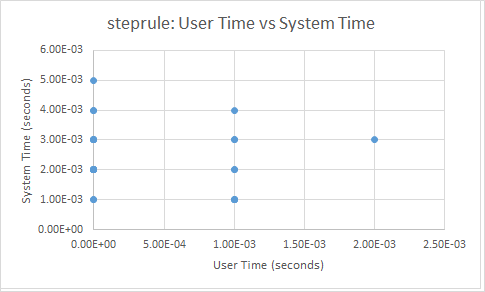
\includegraphics[height=6cm,width=10cm]{steprule.png}
\label{fig:steprule}
\end{figure}

\noindent

The average user time taken by the \textbf{steprule} command was $3.33*10^{-4} s$ with standard deviation $ 5.34*10^{-4}s$. The average system time taken was $2.31 * 10^{-3} s$ with standard deviation $9.80* 10^{-4} s$\\.


\begin{figure}[H] \centering
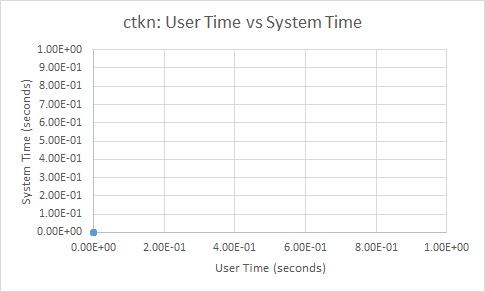
\includegraphics[height=6cm,width=10cm]{ctkn.png}
\end{figure}

\noindent

The average user time taken by the \textbf{ctkn} command was $0 s$ with standard deviation $0 s$. The average system  time taken was $0 s$ with standard deviation $0 s$\\.


\begin{figure}[H] \centering
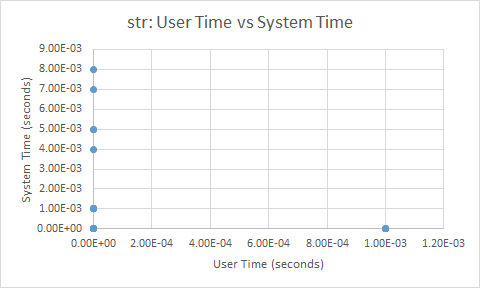
\includegraphics[height=6cm,width=10cm]{str.png}
\end{figure}

\noindent

The average user time taken by the \textbf{str} command was $1.18 * 10^{-4} s$ with standard deviation $3.270 * 10^{-4} s$. The average system  time taken was $1.12 * 10^{-3} s$ with standard deviation $2.1 * 10^{-3} s$\\.


\begin{figure}[H] \centering
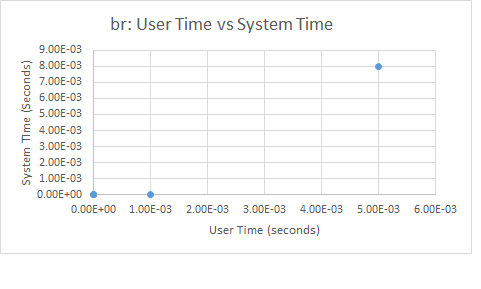
\includegraphics[height=6cm,width=10cm]{br.png}
\end{figure}

\noindent

The average user time taken by the \textbf{br} command was $1.20 * 10^{-3} s$ with standard deviation $2.168 * 10^{-3} s$. The average system time taken was $1.60 * 10^{-3} s$ with standard deviation $3.577 * 10^{-3} s$\\.


\begin{figure}[H] \centering
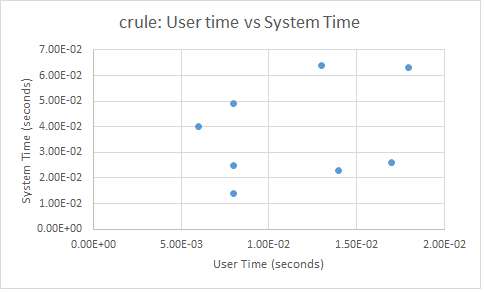
\includegraphics[height=6cm,width=10cm]{crule.png}
\end{figure}

\noindent

The average user time taken by the \textbf{crule} command was $1.15 * 10^{-2} s$ with standard deviation $4.597 * 10^{-3} s$. The average system  time taken was $3.80 * 10^{-2} s$ with standard deviation $1.9046 * 10^{-2} s$\\.

\begin{figure}[H] \centering
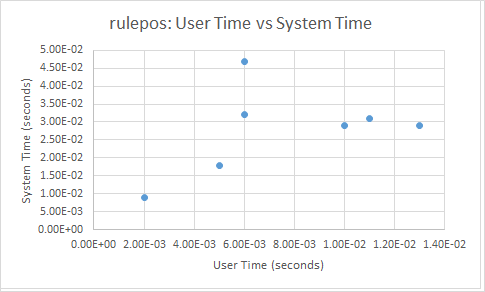
\includegraphics[height=6cm,width=10cm]{rulepos.png}
\end{figure}

\noindent

The average user time taken by the \textbf{rulepos} command was $7.57 * 10^{-3} s$ with standard deviation $3.866 * 10^{-3} s$. The average system time taken was $2.79 * 10^{-2} s$ with standard deviation $1.18930 ^ 10^{-3} s$\\.

\section{Conclusion}

All \verb|sidBison| commands run in either constant or linear time in the average case. While constants might be large, this guarantees that the system's response time will not grow too large as input string sizes increase. Maximum average execution times for grammar are of the order $10^{-3} s$  for $O(1)$ commands and $10^{-2} s$ for $O(n)$ commands, with low standard deviations. If grammar sizes increase, \verb|sidBison|'s command execution time will only grow linearly -- the same as GNU Bison. Thus, debugging tool promises to deliver reasonable execution times for reasonably sized grammars. 

